\documentclass{article}
\usepackage[utf8]{inputenc}
\usepackage{amsmath}
\usepackage{float}
\usepackage{listings}
\usepackage[pdftex]{graphicx}
\usepackage{amssymb}
%--------------------------------------------------------------------

\author{Pratik Aghor}
\title{Fourier and Chebyeshev Spectral Methods for viscous Burger's Equation}
\date{\today}  % Toggle commenting to test

\begin{document}

\maketitle
%--------------------------------------------------------------------
\section{Equation, Notation and Preliminaries:}
%-------------------------------------------------------------------
%-------------------------------------------------------------------
The viscous Burger's equation in $1d$ is as follows:
\begin{equation}\label{eq:burger}
 u_{t} + uu_{x} =  \nu u_{xx}
\end{equation}

A dynamical-systems representation of the same Eqn.(\ref{eq:burger}) is as follows:
\begin{align}\label{eq:burger_abstract}
\begin{split}
 u_{t}  &=  Lu + N(u)\\
 L(u)   &= \nu u_{xx}\\
 N(u)   &= -uu_{x}
\end{split}
\end{align}

The domain $x\in[0, 1]$ is given. In Fourier spectral we will assume periodic boundary conditions (BC's) while in Chebyeshev spectral, Dirichlet BC's are assumed. 

\begin{equation}\label{eq:Dirichlet_BC}
 u(0) = u(1) = 0
\end{equation}


For computational purposes, we will need to transform the physical domain $x \in [0, 1]$ to a computational domain $x_{c} \in [xcmin, xcmax]$. This can be achived via a simple linear transformation given by
\begin{align}\label{eq:x2xc}
 \begin{split}
  x_{c} &= ax + b\\
  b     &= xcmin\\
  a     &= (xcmax-xcmin)
 \end{split}
\end{align}

And to get back from computational domain $x_{c}$ to the physical domain $x$, we need  the inverse of the above transformation:
\begin{equation}\label{eq:xc2x}
 x = (x_{c}-b)/a
\end{equation}


Using chain rule, we can tranform the derivatives with respect to (henceforth wrt) $x$ into derivatives wrt $x_{c}$. 

\begin{align*}
 \begin{split}
  u_{x} &= u_{x_{c}} \frac{dx_{c}}{dx}\\
        &= a u_{x_{c}}\\
  u_{xx}&= \frac{\partial}{\partial x_{c}} \bigg\{u_{x_{c}} \frac{dx_{c}}{dx} \bigg\}\frac{dx_{c}}{dx}\\
        &= a^{2} u_{x_{c} x_{c}}
 \end{split}
\end{align*}

Henceforth, we will use the modified version of the original Eqn(\ref{eq:burger_abstract}) on the computational domain to develop the scheme:

\begin{align}\label{eq:burger_computational}
\begin{split}
 u_{t}  &=  Lu + N(u)\\
 L(u)   &= a^{2}\nu u_{x_{c}x_{c}}\\
 N(u)   &= -a uu_{x_{c}}\\
 N(u)   &= -\frac{a}{2} (u^{2})_{x_{c}}
\end{split}
\end{align}

For time integration, the second-order (two step) Adams-Moulton method for the linear term and the second-order (two-step) Adams-Bashforth method for the nonlinear term are used (Henceforth called AM2AB2).

The AM2AB2 algorithm reads:
\begin{subequations}\label{eq:AM2AB2}
 \begin{equation}
  \frac{u^{n+1}-u^{n}}{\Delta t} = L \frac{u^{n+1} + u^{n}}{2} + \frac{3}{2} N(u^{n}) - \frac{1}{2} N(u^{n-1})
 \end{equation} 
 \begin{equation}
  \bigg( I - \frac{\Delta t}{2} L \bigg) u^{n+1} = \bigg( I + \frac{\Delta t}{2} L \bigg)u^{n} + \frac{3 \Delta t}{2} N(u^{n}) - \frac{\Delta t}{2} N(u^{n-1})
 \end{equation}
\end{subequations}



%-------------------------------------------------------------------
%-------------------------------------------------------------------
\section{Fourier Spectral}
%-------------------------------------------------------------------
%-------------------------------------------------------------------
We begin with developing the formalism from Eqn.(\ref{eq:burger_abstract}). First of all, we need to tranform the physical domain into $x_{c} \in [0, 2\pi]$, where the $c$ stands for `computational'.

From Eqn.(\ref{eq:x2xc}), we get
\begin{align}\label{eq:x2xc_Fourier}
 \begin{split}
  x_{c} &= ax + b\\
  b     &= 0\\
  a     &= 2\pi
 \end{split}
\end{align}

We will try to discretize Eqn.(\ref{eq:burger_computational}) on $x_{c}$. 

Transforming Eqn(\ref{eq:AM2AB2}) into Fourier space by taking a Fourier transform,  AM2AB2 algorithm reads:
\begin{equation}\label{eq:AM2AB2_Fourier}
 \bigg( I - \frac{\Delta t}{2} L \bigg) \hat{u}^{n+1} = \bigg( I + \frac{\Delta t}{2} L \bigg)\hat{u}^{n} + \frac{3 \Delta t}{2} N^{n} - \frac{\Delta t}{2} N^{n-1}
\end{equation}
Where $\hat{u} = FFT(u)$ ,and $N^{n}$ and$N^{n-1}$ are the coefficients in the Fourier tranform of $N(u^{n})$ and $N(u^{n-1})$ respectively.
%-------------------------------------------------------------------
\subsection{Getting fft to work in python}
%-------------------------------------------------------------------
In order to see the oredring of Fourier modes in python, we do some trivial tests.

\begin{align*}
 sin (x) &= \frac{e^{ix} - e^{-ix}}{2i}\\
 cos (x) &= \frac{e^{ix} - e^{-ix}}{2}
\end{align*}

For $N$ grid points, assuming $N$ is even, the Fourier modes $\bar{k} \in [-N/2, N/2]$. In order to find the ordering of $\bar{k}$, we expect to see $ k_{1} = -0.5i$ and $k_{-1} = 0.5 i$ in the expansion of $\sin{x}$. In the expansion of $\cos{x}$, we expect to see $ k_{1} = 0.5$ and $k_{-1} = -0.5$, with all others being zero. 

Some results for different N's are as follows:
\begin{verbatim}
 u = sin(xc) 

N =  8 

v = fft(u) = 
[ 1.43029718e-18+0.00000000e+00j -7.08192362e-17-5.00000000e-01j
  1.53080850e-17-1.38777878e-17j  1.24474906e-17+0.00000000e+00j
  2.91858728e-17+0.00000000e+00j  4.02030662e-17+0.00000000e+00j
  1.53080850e-17+1.38777878e-17j -4.30636606e-17+5.00000000e-01j]
_____________________________________________________________________

u = cos(xc) 

N =  8 

v = fft(u) = 
[-4.30636606e-17+0.00000000e+00j  5.00000000e-01-8.61273212e-17j
  1.53080850e-17+0.00000000e+00j  0.00000000e+00+2.86059436e-18j
  1.24474906e-17+0.00000000e+00j  0.00000000e+00+2.48949813e-17j
  1.53080850e-17+0.00000000e+00j  5.00000000e-01+5.83717456e-17j]
_____________________________________________________________________

u = 2.0*sin(xc) + sin(3.0*xc) 

N =  4 

v = fft(u) = 
[ 1.5308085e-16+0.j  -1.5308085e-16-0.5j  1.5308085e-16+0.j
 -1.5308085e-16+0.5j]

_____________________________________________________________________

u = 2.0*sin(xc) + sin(3.0*xc) 

N =  8 

v = fft(u) = 
[-8.99930287e-17+0.00000000e+00j -1.32051576e-16-1.00000000e+00j
  7.65404249e-17+5.55111512e-17j -1.32051576e-16-5.00000000e-01j
  2.43073879e-16+0.00000000e+00j -2.10292737e-17+5.00000000e-01j
  7.65404249e-17-5.55111512e-17j -2.10292737e-17+1.00000000e+00j]
_____________________________________________________________________
\end{verbatim}

These tests clearly indicate that the $\bar{k}$ is arranged in the following manner:

$\bar{k} = [0, 1, 2, ..., (N/2)-1, N/2, (-N/2)+1, ..., -1]$, i.e., for $N = 8$, 
$\bar{k} = [0, 1, 2, 3, 4, -3, -2, -1]$. There is an obvious asymmetry apparent from this analysis. There is no $k = -4$ mode! If the solution would have been, say, a standing wave, we would never be able to capture it because we will never have enough modes to counter-balance the $k= N/2$ mode. Hence, we decide to forcefully put it to $0$.

From the analysis done in class, we know that the convergence of Fourier spectral method is faster than any algebraic power of $1/N$ (exponential convergence), especially with periodic BC's.

Hence, if we keep enough modes, we can zero-out the highest mode as the coefficients in the expansion of $u$ will drop off fast enough. This way, we keep the $\bar{k}$ symmetric in terms of positive and negative modes present and take $\bar{k} = [0, 1, 2, ..., (N/2)-1, 0, (-N/2)+1, ..., -1]$.

However, because fft assumes periodic BC's we do the calculation on $(N-1)$ grid points where $x_{c} = [0, 2\pi)$, excluding the last grid point. Hence we use $\bar{k} = [0, 1, 2, ..., (N/2)-1, (-N/2)+1, ..., -1]$ in these calculations, removing the redundant higher mode, maintaining the symmetry and $(N-1)$ modes! We pad up the results by writing $u[N-1] = u[0]$, in order to plot the results on the full domain, with the last point included.  
%-------------------------------------------------------------------
\subsection{Results}
%-------------------------------------------------------------------
A sample result obtained for $\nu = 0.01$ was as follows:
  \begin{figure}[H]
        \centering
        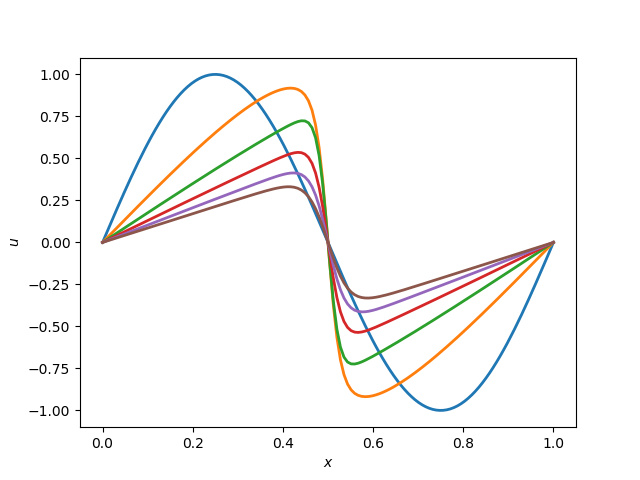
\includegraphics[scale = 0.6]{Figs/ut_fourier.png}
            \caption{$u(t)$ for $\nu = 0.01$}
        \label{fig:ut_fourier_nu_0_01}
\end{figure}

%-------------------------------------------------------------------
%-------------------------------------------------------------------
\section{Chebyshev Spectral}
%--------------------------------------------------------------------
%-------------------------------------------------------------------
We will use the Chebyshev cardinal functions to approximate $u$, i.e., $$u = \sum_{k=0}^{N} u_{k}\psi_{k} $$

where $$\psi_{k} = \frac{(-1)^{k+1}(1-x_{c}^{2})T'_{N}}{\bar{c}_{k} (x_{c}-x_{c_{k}})} $$

with $$\bar{c}_{k} =
    \begin{cases}
      2, & \text{if}\ k=\{0, N\} \\
      1, & \text{otherwise}
    \end{cases}$$
We also assume that the computational grid now is $x_{c} \in [-1, 1]$ with non-uniform grid with grid-points at the Chebyshev-Gauss-Lobatto points.
\begin{equation*}
 x_{j} = \cos{\frac{j \pi}{N}}
\end{equation*}

Evaluating the function at the grid points results in:

\begin{equation*}
 u(x_{j}) = \sum_{k=0}^{N} u_{k}\psi_{k}(x_{j}) = u_{j}
\end{equation*}

%-------------------------------------------------------------------
\subsection{Chebyshev differentiation matrices}
%-------------------------------------------------------------------
As formulated in Prof McHugh's notes and in \cite{trefethen2000spectral}, the Chebyshev differentiation matrix can be formulated as follows:

\begin{equation}
 d_{1jk} = \begin{cases}
      \frac{1+2N^{2}}{6}, & \text{if}\ j = k = 0 \\
      -\frac{1+2N^{2}}{6}, & \text{if}\ j = k = N\\
      -\frac{x_{c_{k}}}{2(1-x_{c_{k}}^{2})}, & \text{if}\ j = k, 0 < k < N \\
      \frac{(-1)^{j+k}\bar{c}_{j} }{\bar{c}_{k}(x_{c_{j}} - x_{c_{k}})}, & \text{if}\ j \neq k \\
    \end{cases}
\end{equation}

This worked well and gave the following result. The grid $x_{c}$ was chosen to be the Chebyshev-Gauss-Lobatto grid and the test function given was $u = \sin{\pi x_{c}}$. The exact derivative is $\pi \cos{\pi x_{c}}$, which matched well with the one obtained from the Chebyshev differentiation matrix.   
  \begin{figure}[H]
        \centering
        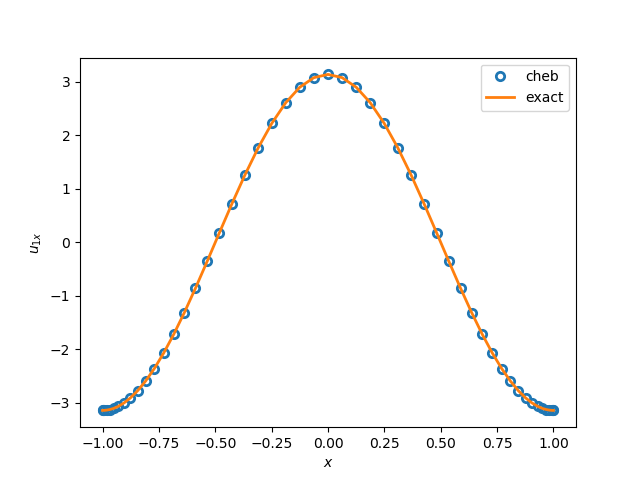
\includegraphics[scale = 0.6]{Figs/test_cheb.png}
            \caption{exact differentiation vs. Chebyshev differentiation of $\sin{\pi x}$}
        \label{fig:test_interpolate_1_c2f}
\end{figure}

%-------------------------------------------------------------------
\subsection{Results}
%-------------------------------------------------------------------
A sample result obtained for $\nu = 0.01$ was as follows:
  \begin{figure}[H]
        \centering
        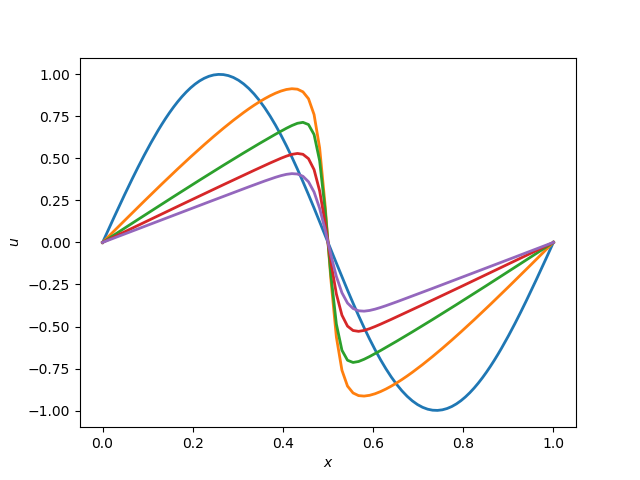
\includegraphics[scale = 0.6]{Figs/ut_cheb.png}
            \caption{$u(t)$ for $\nu = 0.01$}
        \label{fig:ut_fourier_nu_0_01}
\end{figure}

%-------------------------------------------------------------------

%-------------------------------------------------------------------
%--------------------------------------------------------------------
\bibliographystyle{apalike}
%\bibliographystyle{unsrt} % Use for unsorted references  
%\bibliographystyle{plainnat} % use this to have URLs listed in References
%\cleardoublepage
%\bibliography{References/references} % Path to your References.bib file

\bibliography{bib/references} % Path to your References.bib file
 \if@openright\cleardoublepage\else\clearpage\fi
 \cleardoublepage
 \pagestyle{empty}
%--------------------------------------------------------------------
\end{document}
